\documentclass{ximera}

\title{What is a limit?}

\newenvironment{objectives}{\begin{remark}\textbf{Objectives}\\}{\end{remark}}

\begin{document}
\begin{abstract}
\end{abstract}

\subsection{Examples}

Pictured are the graphs of two functions which are continuous for all real numbers. The first is a polynomial and the second is the cosine function.

\begin{center}
    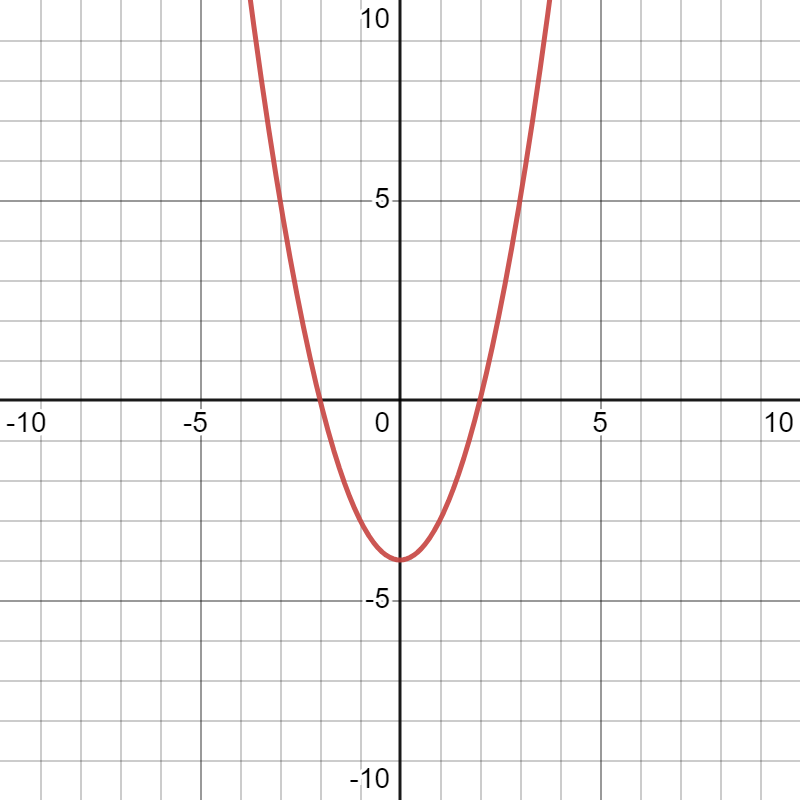
\includegraphics[width=0.75\textwidth]{graph5.png}
\end{center}

Below is an example of a discontinuous graph.

\begin{center}
    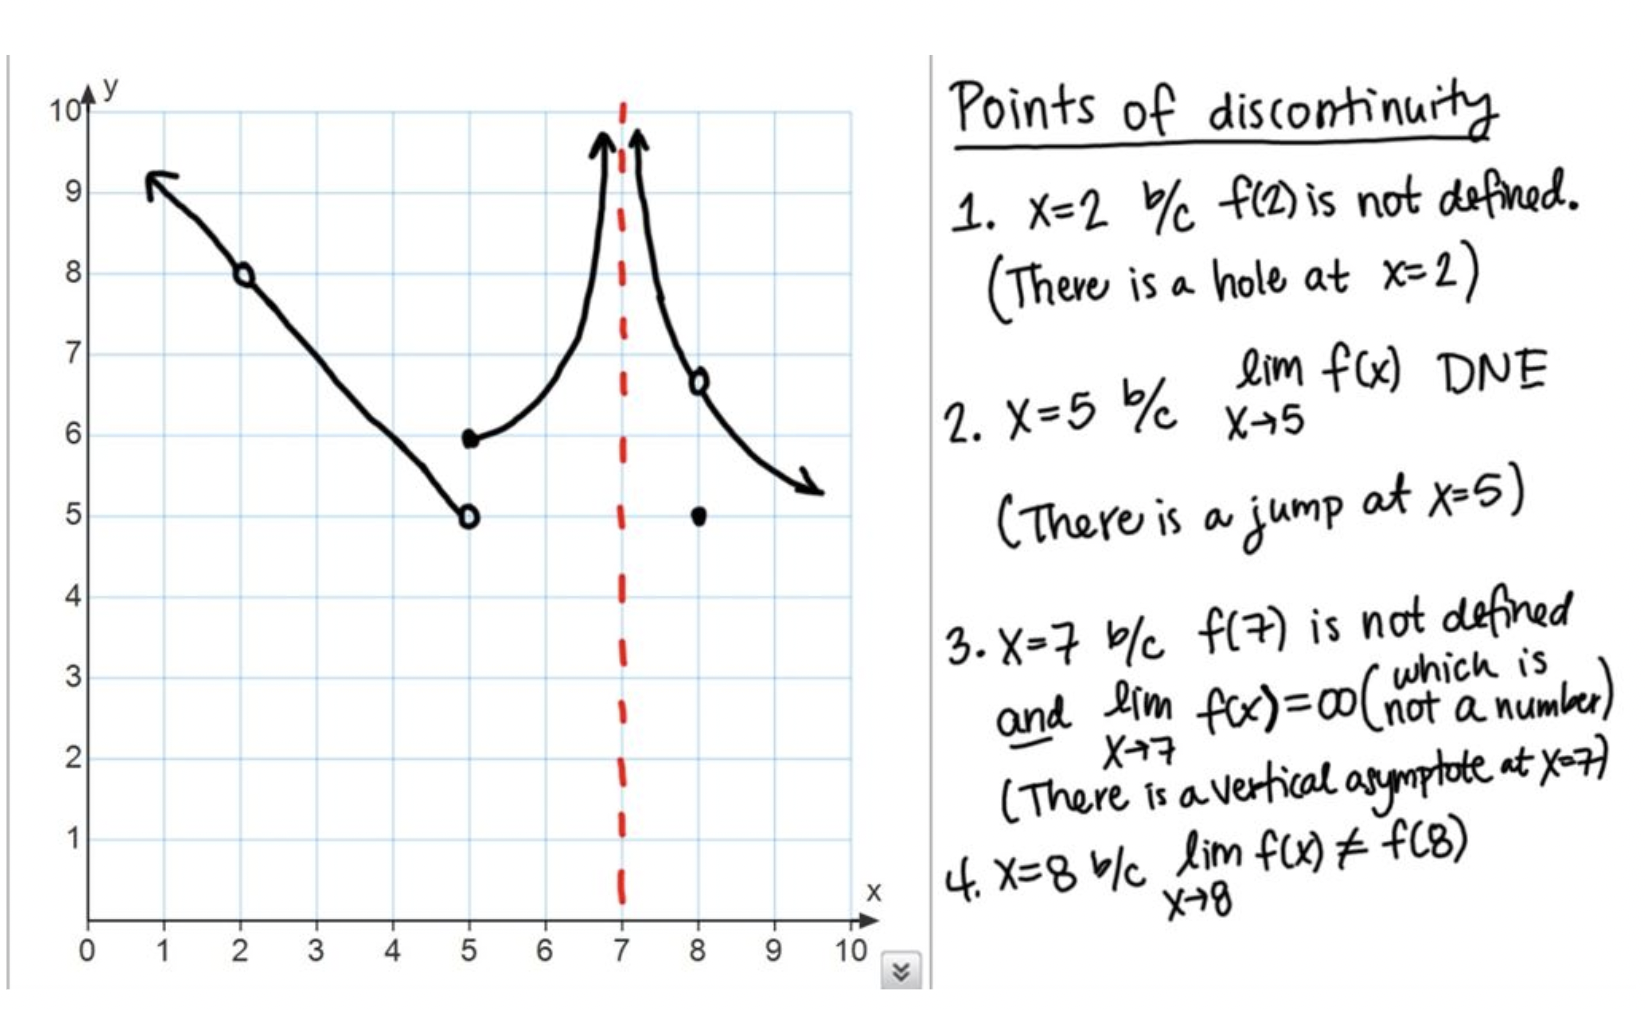
\includegraphics[width=\textwidth]{graph6.png}
\end{center}

\end{document}